\documentclass[11pt,a4paper]{article}

\usepackage[utf8]{inputenc}
\usepackage[T1]{fontenc}
\usepackage{lmodern}
\usepackage[margin=2.5cm]{geometry}
\usepackage{graphicx}
\usepackage{float}
\usepackage{booktabs}
\usepackage{tabularx}
\usepackage{fancyhdr}
\usepackage[hidelinks]{hyperref}

\newcommand{\product}{AI Models Comparator}
\newcommand{\team}{Vivien Gruel \\ Noé Wales \\ Valentin Gempp \\ Maxence Tessier}

\pagestyle{fancy}
\fancyhf{}
\fancyhead[L]{\product}
\fancyhead[R]{Business Requirements Document}
\fancyfoot[C]{\thepage}

\begin{document}

\begin{titlepage}
  \centering
  \vspace*{4cm}
  {\Huge\bfseries \MakeUppercase{\product}\par}
  \vspace{1.5cm}
  {\LARGE Business Requirements Document (BRD)\par}
  \vspace{4cm}
  {\large Software Engineering -- A4 -- 2026-2027\par}
  \vspace{1cm}
  {\large \team\par}
  \vfill
\end{titlepage}

\tableofcontents
\newpage

\section{Project Overview}

\subsection{Project Purpose}

Today, there are a lot of AI models (GPT, Claude, Gemini, Llama, Mistral\dots) and it is hard to know which one is the best. Benchmark results exist, but they are on many different websites. Also, a good benchmark score does not always mean that people like to use the model.

The \product{} is a website that shows two rankings of AI models: one based on benchmark results, and one based on the votes of the users. Each model also has a comment section where users can talk about how the model performs in real life.

\subsection{Project Objectives}

The main objectives of the project are to:
\begin{itemize}
  \item Put the benchmark results of the main AI models in one place.
  \item Let users give their opinion on each model with a simple up or down vote.
  \item Show two rankings (benchmarks and community) and make it easy to see the differences between them.
  \item Give users a place to discuss each model.
  \item Show the latest news about new AI models.
\end{itemize}

\subsection{Business Goals}

\begin{itemize}
  \item \textbf{Help users choose:} users can compare models with real data and with the opinion of other users before they pick one.
  \item \textbf{Save time:} users do not need to check many different websites anymore.
  \item \textbf{Build a community:} votes and comments make people come back and keep the rankings up to date.
\end{itemize}

\subsection{Scope}

The project includes:
\begin{itemize}
  \item \textbf{Model catalogue:} a list of all models, grouped by the lab that created them.
  \item \textbf{Benchmark ranking:} benchmark scores are collected automatically and used to rank the models.
  \item \textbf{Community ranking:} users vote up or down, and the votes are used to rank the models.
  \item \textbf{Comments:} one comment feed for each model.
  \item \textbf{AI news:} news about new models are collected automatically and displayed.
  \item \textbf{Accounts and administration:} sign up, log in, delete an account, and moderation by an administrator.
\end{itemize}

\noindent\textbf{Not included:} running the models, running benchmarks ourselves, price comparison, a mobile app, and replies to comments.

\section{Stakeholder Analysis}

\subsection{Key Stakeholders}

\begin{itemize}
  \item \textbf{Visitors:} people who look at the website without an account.
  \item \textbf{Registered users:} developers, students and AI fans who vote and write comments.
  \item \textbf{Administrators:} they moderate the comments and the users, and they check that the data imports work.
  \item \textbf{Data providers:} the websites that publish benchmark results and AI news.
  \item \textbf{Development team:} the four students who build and maintain the application.
  \item \textbf{TD instructor:} validates the project and grades the deliverables.
\end{itemize}

\subsection{Stakeholder Needs}

\begin{itemize}
  \item Visitors want to see quickly which models are the best, without creating an account.
  \item Registered users want an easy way to give their opinion and to talk with other users.
  \item Administrators need simple tools to delete bad comments and block users who do not respect the rules.
  \item Data providers want their data to be used correctly, with their name displayed.
  \item The development team needs a project that can be finished during the sprints of the course.
\end{itemize}

\section{Business Requirements}

\subsection{Functional Business Requirements}

\begin{description}
  \item[BR-1] \textbf{Model Catalogue}
  \begin{itemize}
    \item The system must show all the models grouped by lab, with the name and the logo of each lab, in alphabetical order.
    \item Each model must have its own page with its lab, release date, benchmark scores, rankings, votes and comments.
  \end{itemize}
  \item[BR-2] \textbf{Benchmark Ranking}
  \begin{itemize}
    \item The system must collect benchmark scores automatically from external websites and show where each score comes from.
    \item The system must rank the models by their benchmark results. A model with not enough benchmarks is shown as ``not ranked''.
  \end{itemize}
  \item[BR-3] \textbf{Community Ranking}
  \begin{itemize}
    \item A registered user must be able to vote up or down for each model, change the vote, or remove it.
    \item The system must rank the models by their percentage of up votes. A model with not enough votes is shown as ``not ranked''.
  \end{itemize}
  \item[BR-4] \textbf{Ranking Comparison}
  \begin{itemize}
    \item Users must be able to switch between the two rankings. Each line must also show the position of the model in the other ranking.
  \end{itemize}
  \item[BR-5] \textbf{Comments}
  \begin{itemize}
    \item Each model must have a comment feed, with the newest comment on top. Registered users can post as many comments as they want.
    \item Users must be able to delete their own comments.
  \end{itemize}
  \item[BR-6] \textbf{AI News}
  \begin{itemize}
    \item The system must collect news about AI models automatically and show them from the newest to the oldest, with a link to the original article.
  \end{itemize}
  \item[BR-7] \textbf{User Accounts}
  \begin{itemize}
    \item Visitors must be able to create an account and log in. Users must be able to delete their account.
  \end{itemize}
  \item[BR-8] \textbf{Administration}
  \begin{itemize}
    \item Administrators must be able to delete any comment, block, unblock or delete a user, and see if the data imports work.
  \end{itemize}
\end{description}

\subsection{Non-Functional Business Requirements}

\begin{description}
  \item[NBR-1] \textbf{Usability:} the website must be easy to use without any training, and every page must work on a phone (360\,px wide screen).
  \item[NBR-2] \textbf{Performance:} each page must load in less than 2 seconds with up to 100 users at the same time.
  \item[NBR-3] \textbf{Availability:} if an external website is down, the application must still work and show the last data it received.
  \item[NBR-4] \textbf{Security:} passwords must be hashed, all communications must use HTTPS, and only administrators can access the administration features.
  \item[NBR-5] \textbf{Maintainability:} it must be possible to add a new benchmark or news source without changing the rest of the application.
\end{description}

\subsection{Compliance Requirements}

\begin{itemize}
  \item \textbf{GDPR:} we only store the email, the username and the hashed password. Users must accept the privacy policy when they sign up. When an account is deleted, all its votes and comments are deleted too.
  \item \textbf{Data sources:} we respect the terms of use of each external website and we display its name in the application.
\end{itemize}

\section{Functional Requirements Mapping}

\subsection{Mapping Business Requirements to Functional Requirements}

\begin{center}
\begin{tabularx}{0.8\textwidth}{lX}
  \toprule
  \textbf{Business requirement} & \textbf{SRS section} \\
  \midrule
  BR-1 Model Catalogue & 3.1.1 \\
  BR-2 Benchmark Ranking & 3.1.2 \\
  BR-3 Community Ranking & 3.1.3 \\
  BR-4 Ranking Comparison & 3.1.4 \\
  BR-5 Comments & 3.1.5 \\
  BR-6 AI News & 3.1.6 \\
  BR-7 User Accounts & 3.1.7 \\
  BR-8 Administration & 3.1.8 \\
  \bottomrule
\end{tabularx}
\end{center}

\section{Business Process Flow}

The diagram below shows the main information that goes between the application, its users and the external websites.

\begin{figure}[H]
  \centering
  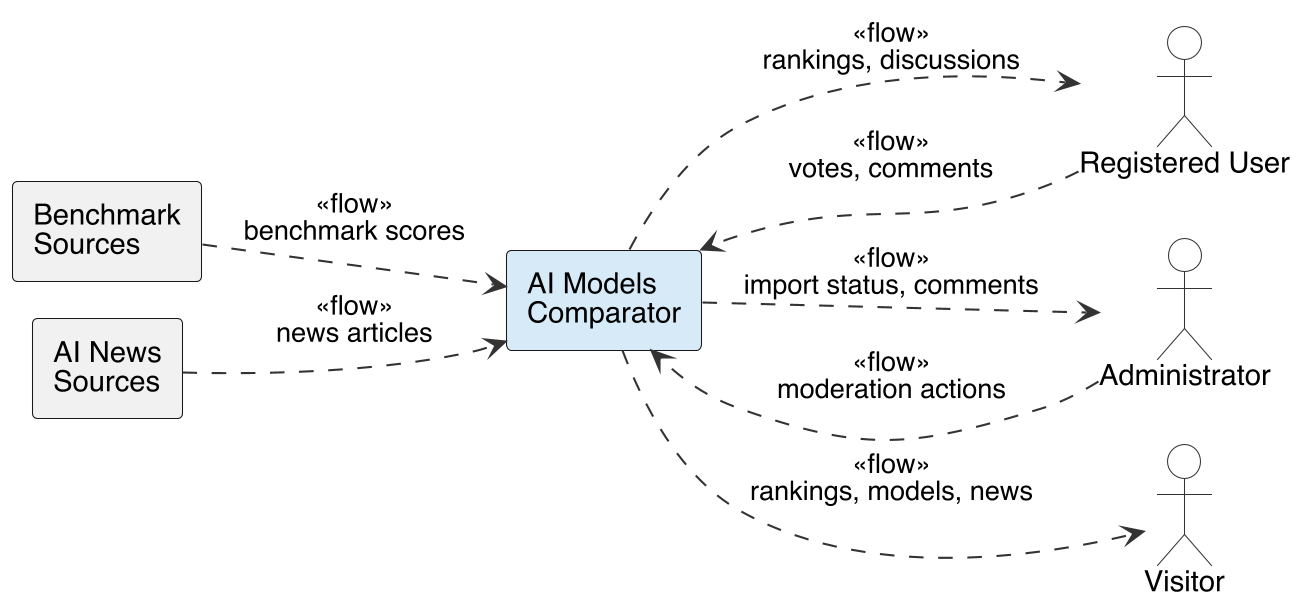
\includegraphics[width=0.9\textwidth]{figures/information-flow.png}
  \caption{Information flow diagram}
\end{figure}

\subsection{Registration and Login}

\begin{enumerate}
  \item \textbf{Process:} a visitor creates an account or logs in. A blocked account cannot log in.
  \item \textbf{Inputs:} email, username, password, acceptance of the privacy policy.
  \item \textbf{Outputs:} a new active account, or an open user session.
\end{enumerate}

\begin{figure}[H]
  \centering
  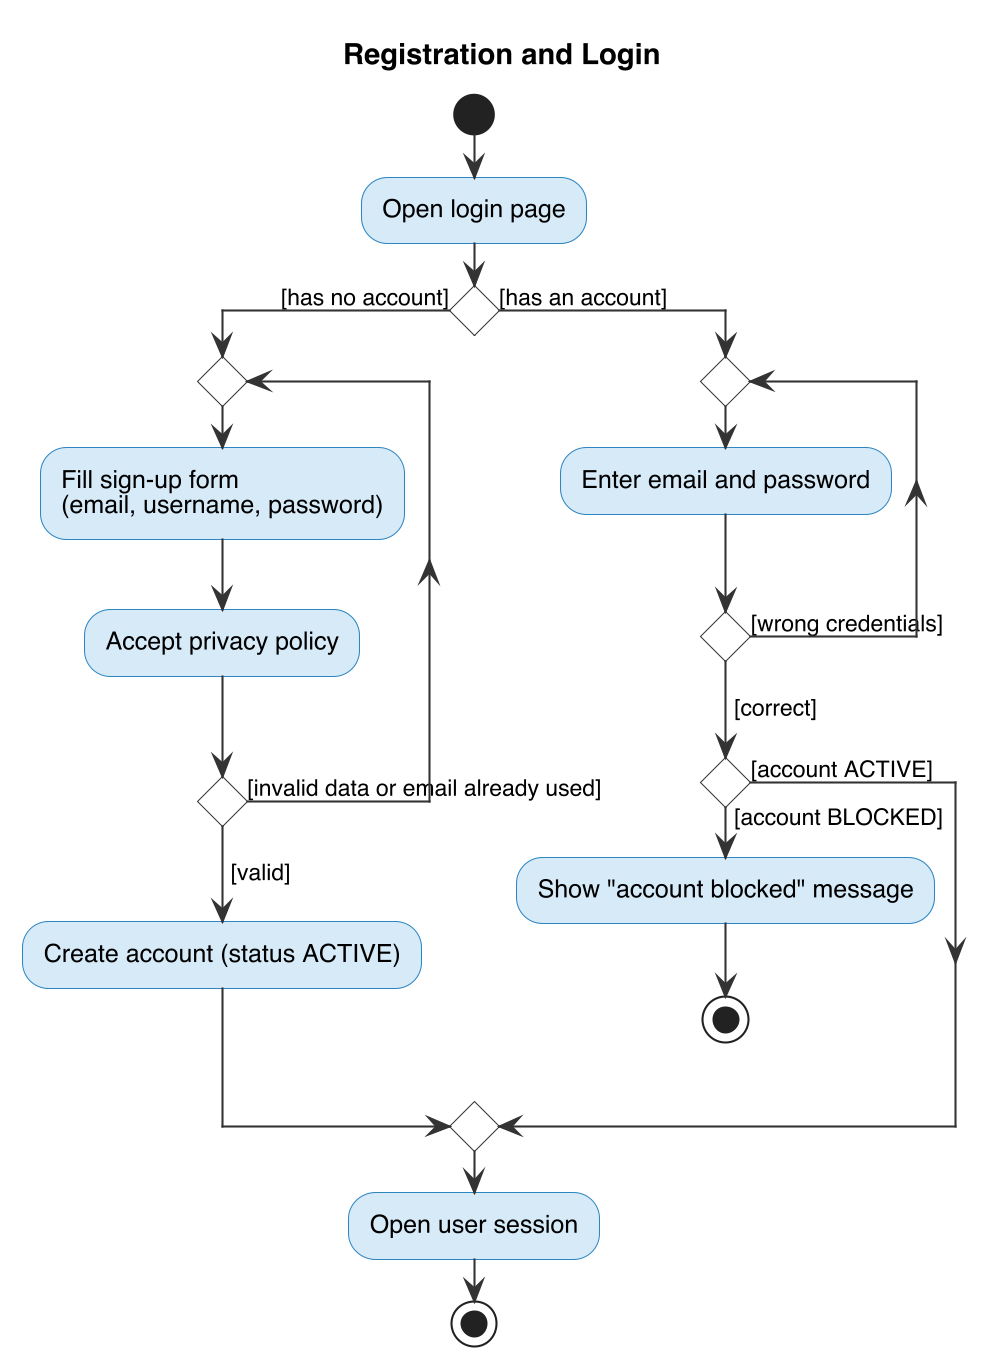
\includegraphics[width=\textwidth,height=0.55\textheight,keepaspectratio]{figures/registration.png}
  \caption{Activity diagram of registration and login}
\end{figure}

\subsection{Voting for a Model}

\begin{enumerate}
  \item \textbf{Process:} a logged-in user opens the page of a model and votes up or down. If the user clicks the same arrow again, the vote is removed. If the user clicks the other arrow, the vote is changed.
  \item \textbf{Inputs:} user session, model, vote direction.
  \item \textbf{Outputs:} saved vote, new community score and ranking.
\end{enumerate}

\begin{figure}[H]
  \centering
  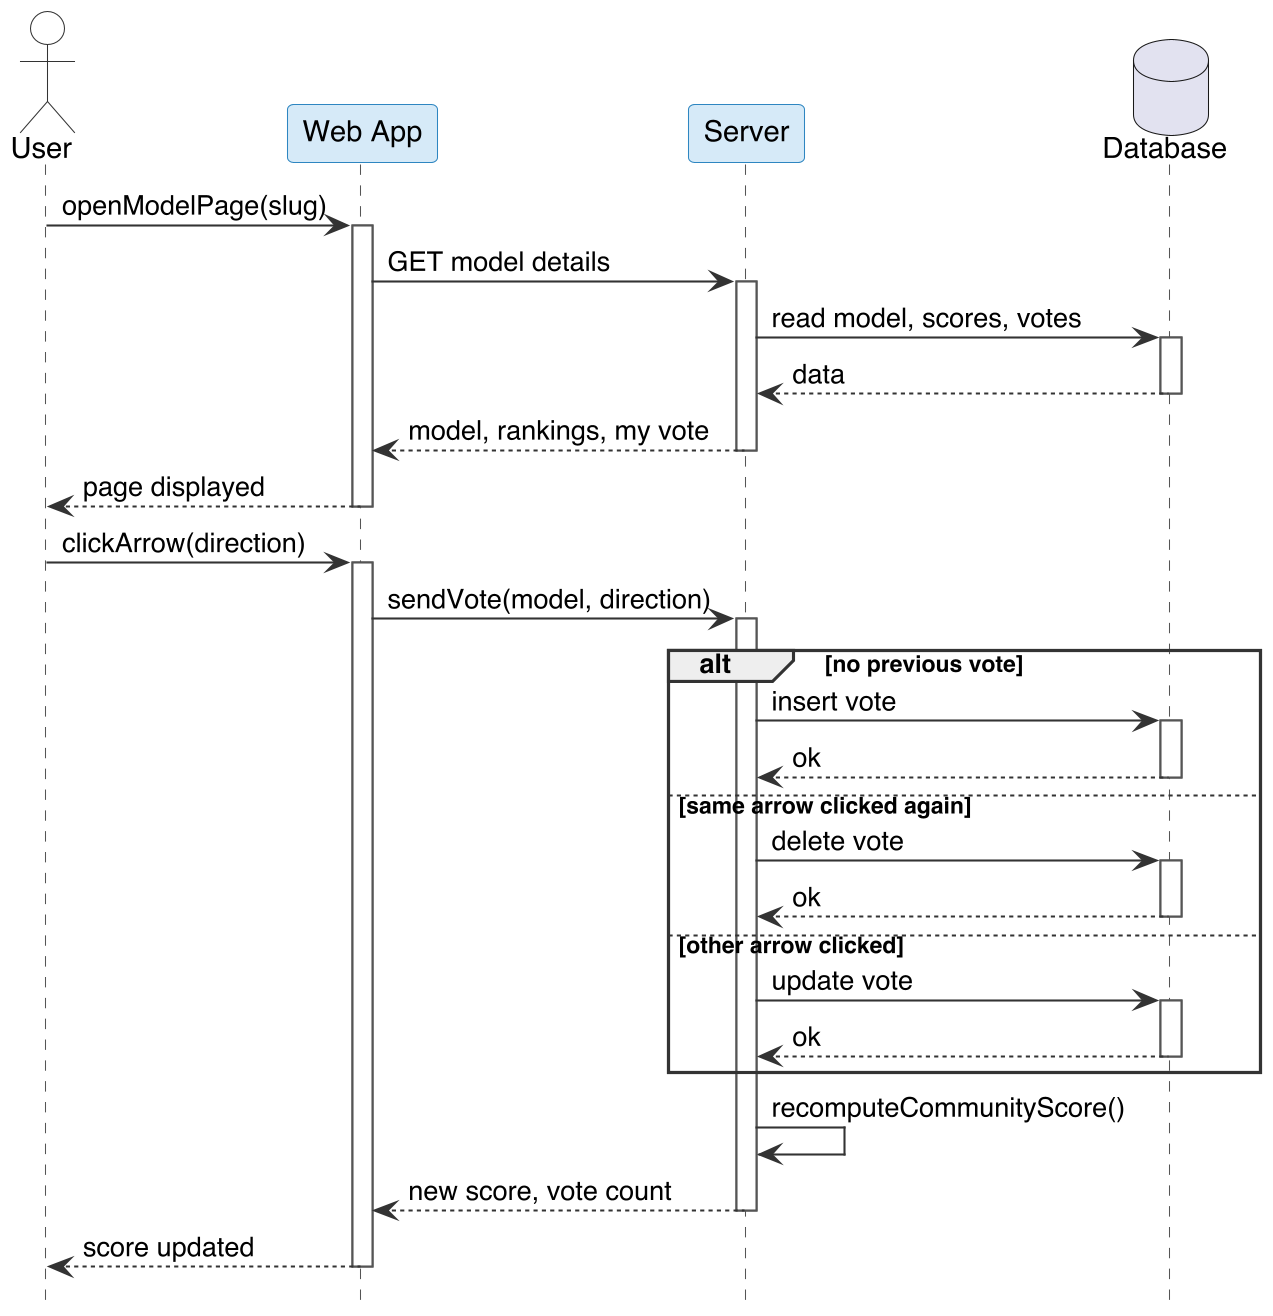
\includegraphics[width=\textwidth,height=0.55\textheight,keepaspectratio]{figures/voting.png}
  \caption{Sequence diagram of the voting process}
\end{figure}

\subsection{Comment Moderation}

\begin{enumerate}
  \item \textbf{Process:} a user publishes a comment. An administrator checks the recent comments and deletes the bad ones. If the author does it again, the administrator also blocks the author.
  \item \textbf{Inputs:} published comments, decision of the administrator.
  \item \textbf{Outputs:} deleted comment, and blocked account if needed.
\end{enumerate}

\begin{figure}[H]
  \centering
  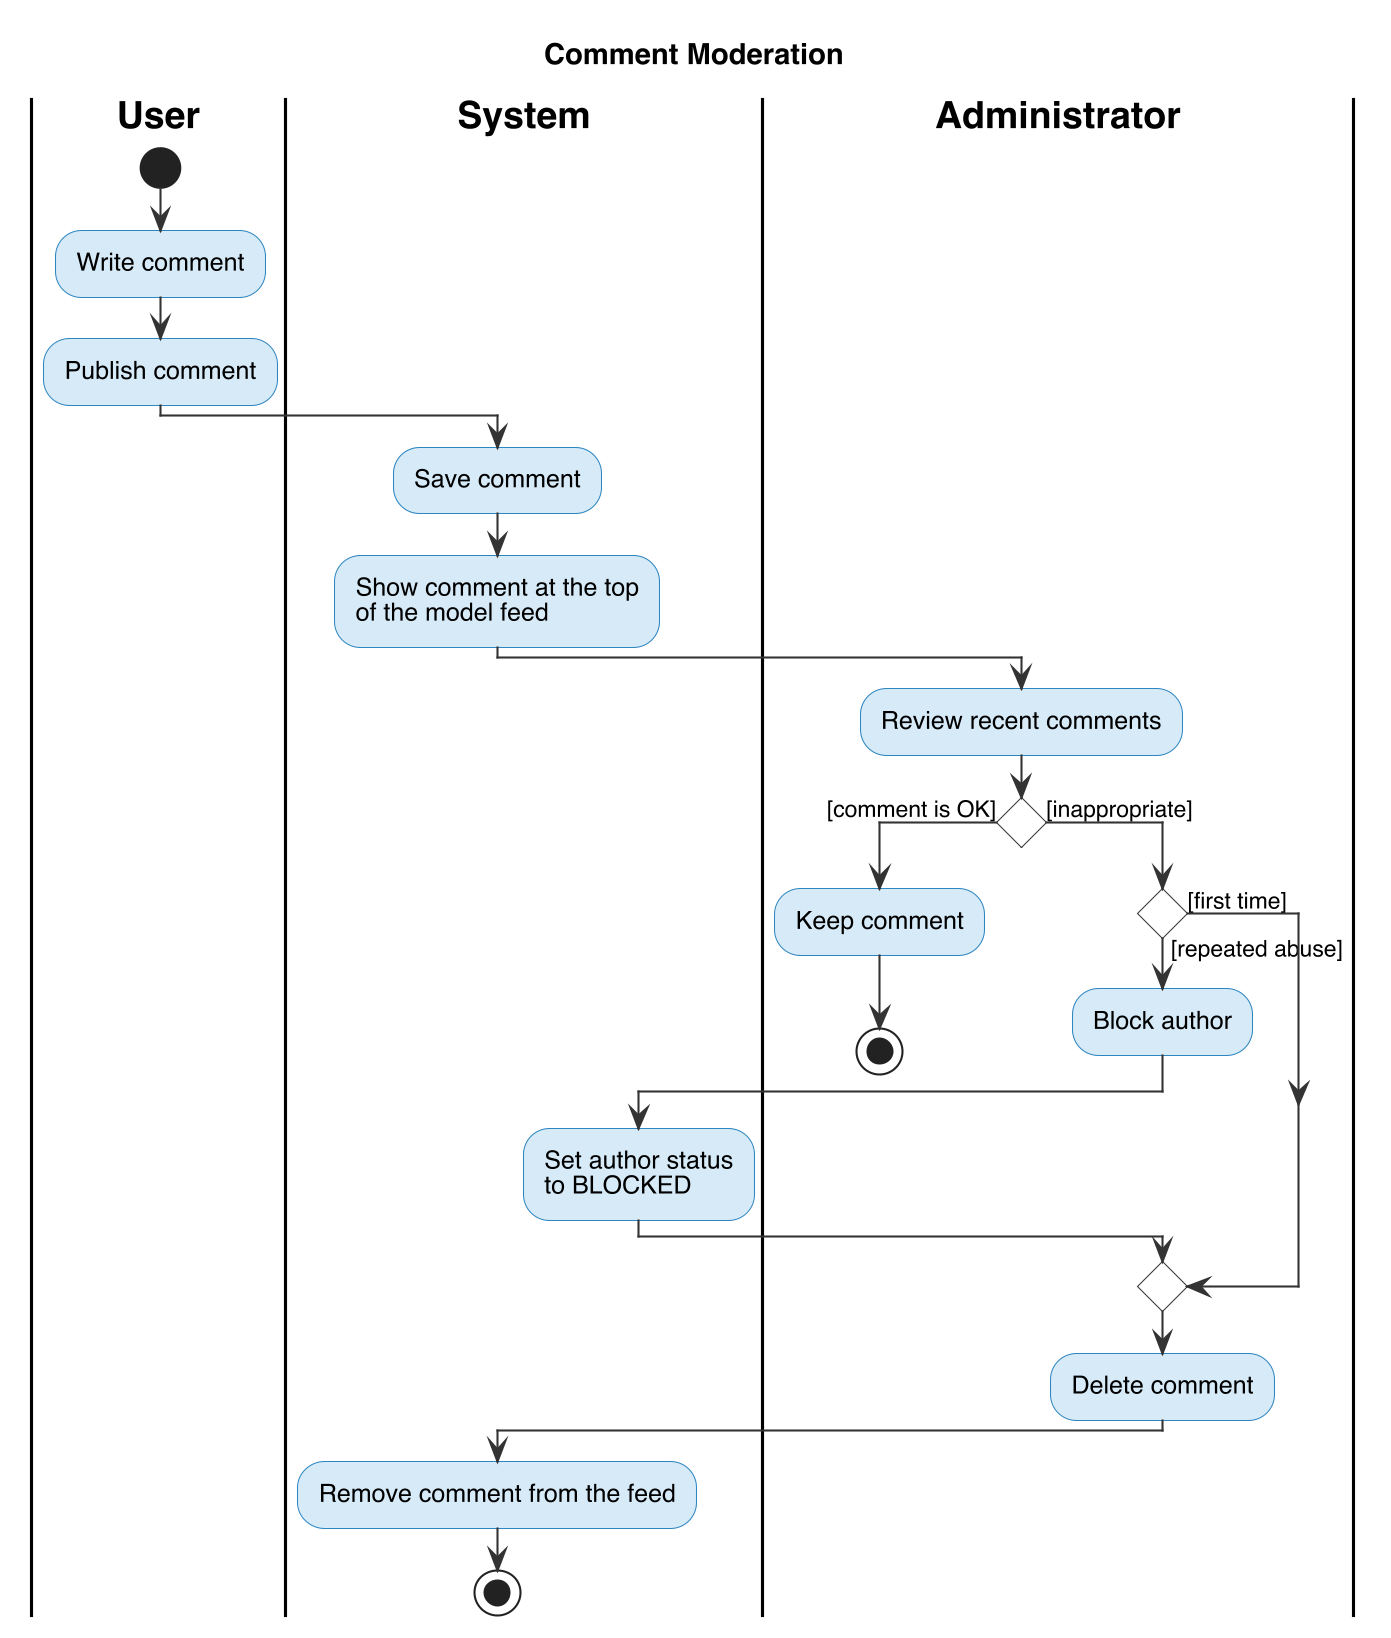
\includegraphics[width=\textwidth,height=0.6\textheight,keepaspectratio]{figures/moderation.png}
  \caption{Activity diagram of comment moderation (with swimlanes)}
\end{figure}

\section{Risks and Assumptions}

\subsection{Risks}

\begin{itemize}
  \item \textbf{Source not available:} an external website can change its format, block the access or close.
  \item \textbf{Different model names:} websites do not always use the same name for the same model, so some scores can be missing or linked to the wrong model.
  \item \textbf{Fake votes:} one person can create many accounts to push a model up or down.
  \item \textbf{Bad comments:} some comments can contain insults, spam or advertising.
  \item \textbf{Not enough users:} with few votes, the community ranking does not mean much.
\end{itemize}

\subsection{Assumptions}

\begin{itemize}
  \item At least one public website gives benchmark scores for the main models, with an API or a file we can download.
  \item At least one free source gives news about AI models.
  \item Users have a recent web browser and an internet connection.
\end{itemize}

\section{Implementation Strategy}

\subsection{Phased Implementation}

\begin{enumerate}
  \item \textbf{Phase 1:} model catalogue, benchmark import and benchmark ranking.
  \item \textbf{Phase 2:} user accounts, votes, community ranking and comments.
  \item \textbf{Phase 3:} administration, AI news and final tests.
\end{enumerate}

\subsection{Training and Support}

\begin{itemize}
  \item Visitors and users do not need training: the website must be easy to understand.
  \item A short guide explains to administrators how to moderate and how to check the imports.
\end{itemize}

\section{Success Criteria}

\begin{itemize}
  \item \textbf{Catalogue:} at least 30 models from at least 5 labs.
  \item \textbf{Benchmarks:} at least 80\,\% of the models are in the benchmark ranking.
  \item \textbf{Performance:} every page loads in less than 2 seconds.
  \item \textbf{Reliability:} at least 95\,\% of the automatic imports work.
  \item \textbf{Usability:} all the user actions can be done on a phone screen (360\,px wide).
\end{itemize}

\section{Approval and Sign-off}

This document is reviewed and approved by:
\begin{itemize}
  \item Development Team: Vivien Gruel, Noé Wales, Valentin Gempp, Maxence Tessier
\end{itemize}

\end{document}
